%----------------------------------------------------------
\chapter{Программная реализация}\label{chap3_soft_architecture}
%----------------------------------------------------------
\subsection{Создание примитивов на странице}
Как было ранее сказано, редактор графов является web-приложением написанным на языке JavaScript. Для создания графа необходима возможность создавать простейшие примитивы: окружности, линии и прочее. JavaScript предоставляет несколько вариантов для решения этой задачи:
\begin{itemize}
	\item Использование HTML -- элемента canvas
	\item Работа с векторной графикой svg
\end{itemize}
Использование сanvas не подходит поскольку после создания примитива невозможно получить его свойства, а следовательно и отредактировать их. Таким образом, необходимо работать с векторной графикой svg, использование svg позволяет создавать примитивы, которые создаются как HTML теги с набором свойств, что позволяет редактировать или удалять созданные примитивы. Однако работать с svg без использования сторонних библиотек достаточно затруднительно, программный код сильно увеличивается и разработка функций для отрисовки примитивов занимает существенно больше времени. Для решения этой задачи подходит библиотека d3.js. Библиотека предоставляет набор инструментов для визуализации данных на странице, который состоит из нескольких дестяков небольших модулей, каждый из которых решает свою задачу. В программном коде возможности d3 используются для создания svg примитивов на странице, например создание вершины (листинг~\ref{lst:gm.exmpl.1}).

\begin{lstlisting}[label={lst:gm.exmpl.1}, caption={Пример создание вершины с использование библиотеки d3}, language=JavaScript]
  svg
    .append("circle")
    .attr("cx", x)
    .attr("cy", y)
    .attr("r", radius)
    .attr("stroke-width", borderWidth)
    .attr("id", id)
    .attr("fill", "#FFFFFF")
    .attr("stroke", "#000000")
    .attr("class", "vertex");
\end{lstlisting}

\subsection{Хранение информации о графовой модели}
Для того, чтобы иметь возможность гибко редактировать графовую модель, а также иметь возможность экспортировать граф в формат aDOT, необходимо хранить множество свойств графа. Так, при удалении вершины, помимо удаления примитивов со страницы, необходимо удалить всю информацию о вершине и связанных с ней ребрах, в противном случае при сохранении графа в формате aDOT в файле будет содержаться информация об уже удаленных вершинах или ребрах.

Все свойства графа хранятся в оперативной памяти. Для хранения большей части свойств в программном коде используются объекты. Объект - это мощная структура данных в javascript - используется для хранения коллекций разных значений. Рассмотрим на примере как храниться информаци о вершинах. В рассматриваемом примере (листинг~\ref{lst:gm.exmpl.2}) представлены хранимые в объекте свойства одной вершины из которой выходит одно ребро.

\begin{lstlisting}[label={lst:gm.exmpl.2}, caption={Пример хранение вершины в оперативной памяти}, language=JavaScript]
{
    "edges": [
        {
            "direction": "from",
            "function": "f1",
            "predicate": "p1",
            "label": "<p1, f1>",
            "metadata": {
                "edgeID": "edge1",
                "pathID": "edge1_path",
                "labelID": "edge1_label",
            }
            "type": "straight",
            "value": "vertex2",
        },
    ],
    "metadata": {
        "label": "s1",
        "label_metadata": {
            "pathID": "vertex1_path",
            "labelID": "vertex1_label",
        },
        "position": {
            "x": 227.609375,
            "y": 211,
        },
    }
}
\end{lstlisting}

Аналогичным образом с помощью объектов храниться информация о предикатах и функциях, которые пользователь вводит в процессе создания графовой модели. Для хранения более простых блоков данных используются массивы, например, хранение позиций уже созданных вершин, или хеш-таблицы, например, хранение уже созданных меток вершин.

\subsection{Поиск циклов в графовой модели}
Разработанный редактор позволяет найти циклы в создаваемой или загружаемой графовой модели. Для поиска циклов в графе реализован алгоритм в основе которого лежит DFS(Depth-first search) - поиск в глубину. Алгоритм является рекурсивным: для рассматриваемой вершины необходимо перебрать все ребра, которые выходят из нее, если ребро приходит в нерасмотренную ранее вершину, то алгоритм запускается от этой вершины. Возврат происходит в том случае, если все выходящие из рассматриваемой вершины ребра идут в уже расмотренные ранее вершины. В результате работы алгоритма будут рассмотрены все вершины графа. 

Стоит обратить внимание, что в интернете представлено множество различных реализаций поиска циклов в графе, однако почти все предложенные реализации выполняют проверку графа на ацикличность, то есть нахождение любого цикла в графе с последующим утверждением, что граф цикличен или ацикличен в противном случае. В то время как в разработанном редакторе необходимо найти все циклы в графе. В основе реализованного алгоритма также лежит DFS, а для нахождения всех циклов в графе поиск в глубину запускается от всех нерасмотренных ранее вершин. Алгоритм состоит из двух функций: функция для поиска в глубину и соответственно вызывающая функция. 
Далее на рисунках (\ref{fig:example_main_dfs}) и (\ref{fig:example_process_dfs}) приведены блок-схемы этих функций.

\begin{figure}[ht!]
\center{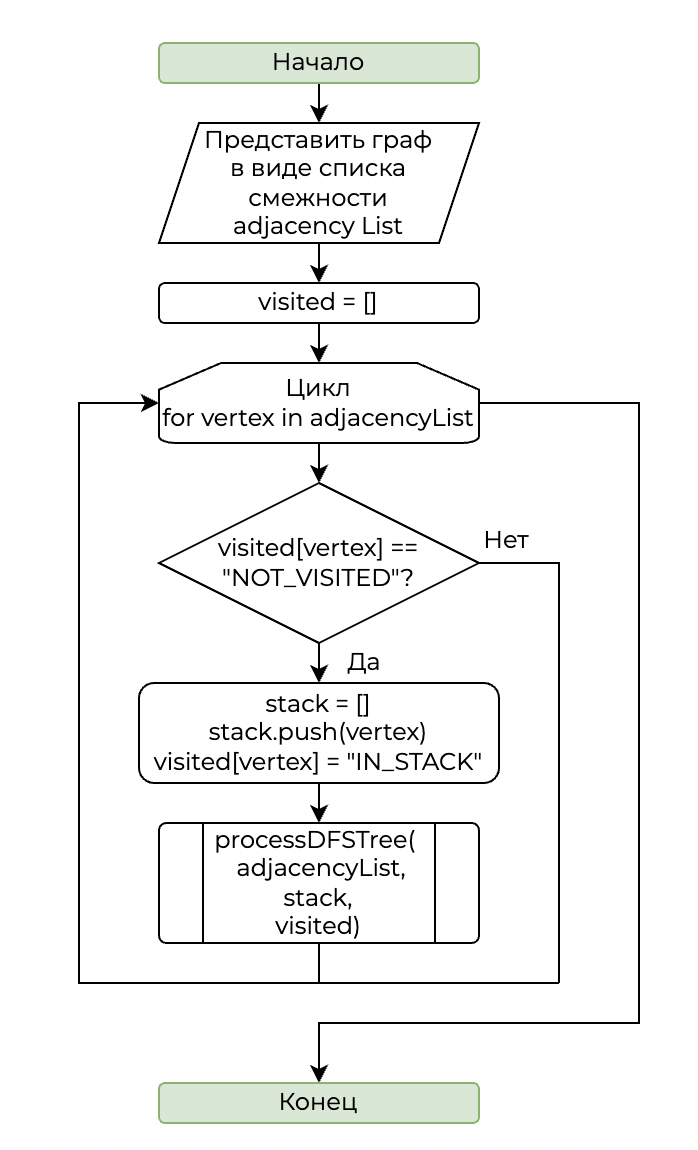
\includegraphics[width=0.4\linewidth]{images/main_dfs.png}}
\caption{Главная функция алгоритма поиска циклов в графе}
\label{fig:example_main_dfs}
\end{figure}

\begin{figure}[ht!]
\center{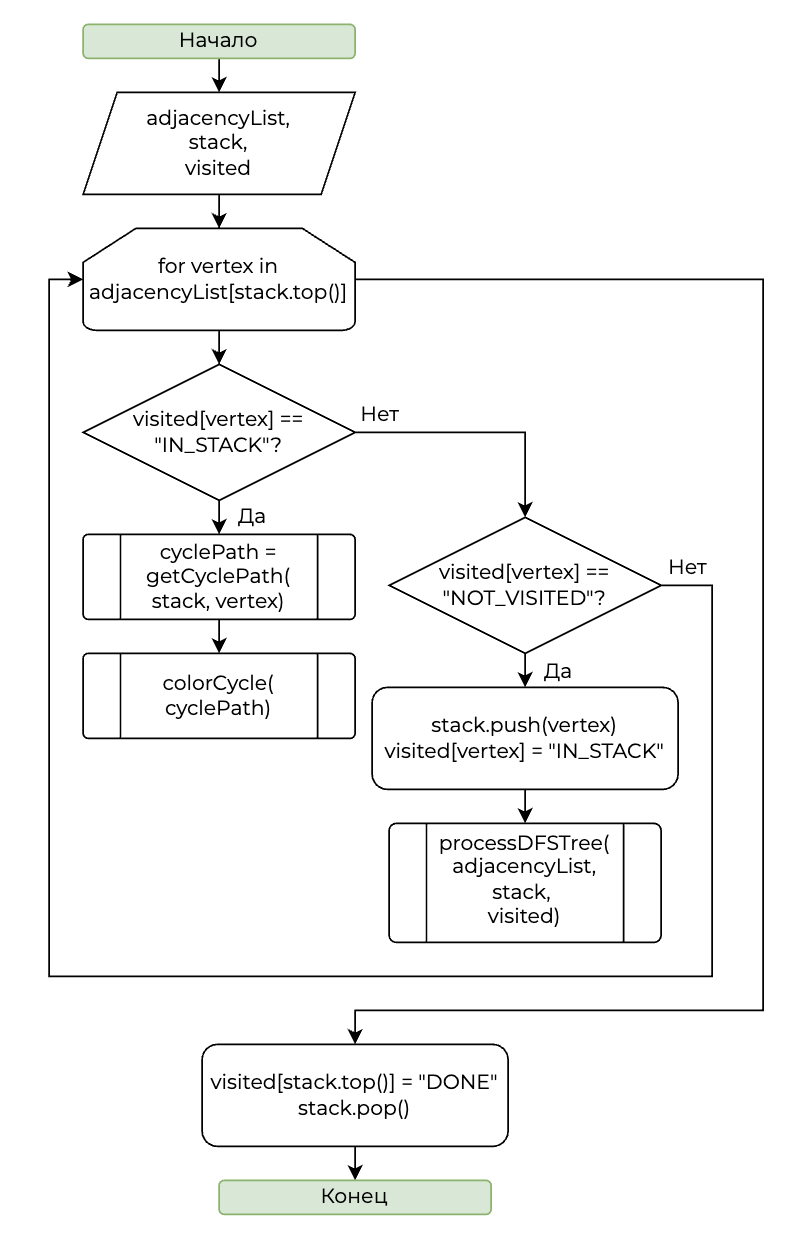
\includegraphics[width=0.4\linewidth]{images/process_dfs.png}}
\caption{Функция выполняющая обход в глубину}
\label{fig:example_process_dfs}
\end{figure}

Разработанный алгоритм позволяет находить все циклы в графе и выполнять из подсветку. В следующем разделе приведены примеры работы алгоритма на разных графовых моделях.
